\clearpage
\chapter{\textbf{Stand der Technik für Anwesenheitserkennung/-prognose}}\label{grundlagen}
%\addtocontents{toc}{\vspace{0.5cm}}

Man kann verschiedene Techniken zur Anwesenheitserkennung und -prognose in Innenräumen in \textit{aktive} und
\textit{passive} Verfahren unterteilen. \\\\
%\section{Aktive und Passive Messverfahren}
Aktive Verfahren messen die menschliche Anwesenheit etwa mit 
Kamera- oder Infrarotsensoren, welche den Menschen direkt im Raum erkennen können. Ein Kamerasensor nimmt
dabei kontinuierlich Bilder des Raumes auf, während ein Algorithmus im Hintergrund versucht ein 3D-Modell 
eines menschlichen Skeletts auf sich bewegende Teile des Bildes zu legen. Bewegen sich über mehrere Bilder 
hinweg die Bereiche auf und unmittelbar neben dem 3D-Modell, registriert das System eine Anwesenheit.\\\\
Infrarotsensoren dagegen funktionieren eher wie ein klassischer Bewegungsmelder, welcher Unterschiede in der 
Infrarotstrahlung eines Raumes erkennt. Durch die generierte Körperwärme des menschlichen Körpers verursacht 
ein Mensch, der sich durch den Sensor bewegt, einen Ausschlag des Sensors.\\

Passive Verfahren orientieren sich an den physikalischen Eigenschaften des Raumes. Anstatt die Präsenz des 
Menschen direkt zu messen, wird versucht, diese anhand von Veränderungen der Eigenschaften der Raumluft oder 
elektromagnetischer Strahlung des Raumes zu erkennen. \\
Verändert sich beispielsweise durch menschliche Anwesenheit die Luftfeuchtigkeit 
in einem Raum in sehr geringem Maß, wird die  Laufzeit einer Ultraschallwelle, die durch diesen Raum 
geschickt wird, leicht verringert, da die Schallgeschwindigkeit in dichteren Medien zunimmt.\\
Die Systeme unterscheiden sich neben der Art der Messung auch deutlich in der Komplexität der Implementierung.
Während Ultraschallsensoren wegen der verhältnismäßig geringen Schallgeschwindigkeit keine besonders hohe 
Genauigkeit besitzen müssen, sind die an einen Mikrowellensensor gestellten Ansprüche wesentlich höher, da sich
Mikrowellen mit deutlich höherer Geschwindigkeit im Raum ausbreiten. Mikrowellen erreichen in Atemluft Geschwindigkeiten
von ca. $300\cdot10^6 \,m/s$, Schallwellen lediglich ca. $330\, m/s$.
Mit Mikrowellen können Bewegungen durch Ausnutzung des Doppler-Effektes einer elektromagnetischen Welle erkannt 
werden. Bewegen sich Objekte oder Personen auf den Sensor zu, wird das Echo der Welle gestaucht, wodurch die 
Bewegung erkannt wird.\\
Hier verdeutlicht sich nochmals die Motivation dieser Arbeit, da Sensoren für Temperatur, Luftfeuchtigkeit oder CO2
weder teuer sind, noch besondere Ansprüche an Positionierung im Raum oder Kalibrierung besitzen.

\chapter{\textbf{Untersuchte Verfahren}}

\section{Machine Learning}\label{unterkapitel}
\addtocontents{toc}{}%\vspace{0.8cm}}

Machine Learning ist ein Teilbereich der künstlichen Intelligenz und beschreibt das Entwickeln mathematischer 
Modelle zur statistischen Auswertung von Daten.\\
Dabei wird dem Modell anhand von Trainingsdaten beigebracht, Gesetzmäßigkeiten zu erkennen, um danach Erwartungen 
über bisher unbekannte Daten treffen zu können.  
Beispielsweise könnte ein solches Modell aus einem Datenset mit aktueller Jahreszeit, Uhrzeit und 
Position der Sonne am Himmel trainiert werden, sodass es schließlich auch in einem anderen Datenset 
aus Jahreszeit und Position der Sonne Rückschlüsse auf die Uhrzeit treffen kann.\\
Als Vorbild für diesen ,,Lernvorgang'' dient das menschliche Gehirn, welches ebenfalls versucht zwischen 
bestimmten Input-Parametern wie z.B. Form und Farbe eines Gegenstandes eine Beziehung herzustellen,
um das beobachtete Objekt in Zukunft schneller kategorisieren zu können.\\
Da eine Vielzahl von effektiven Machine Learning Algorithmen existiert, ist es essenziell, sich mit den
Stärken und Schwächen einzelner Herangehensweisen zu befassen.\\

In dieser Arbeit sollen zwei Unterkategorien des Machine Learning genauer betrachtet werden:
\begin{itemize}
    \item \textit{Supervised Learning} 
    \item \textit{Unsupervised Learning}
\end{itemize}
\textit{Supervised Learning} bedeutet zwischen bestimmten Feldern eines Datensets eine Beziehung
zu einem sog. Label herzustellen, welches als eine Art Ergebnis aus den Eingabewerten gesehen 
werden kann. Ein so trainiertes Modell kann dann neue, ihm vorher unbekannte Datensets, mit einem 
Label versehen - etwa wie in dem o.g. Beispiel, wo Jahreszeit und Sonnenposition die Eingabewerte 
und die Uhrzeit das Label darstellen. Der Begriff ,,\textit{supervised}'' ergibt sich daraus, dass 
das Datenset, mit dem das Modell trainiert wird, diese Labels gegeben 
hat, sodass das Modell sich bei jedem Schritt des Lernvorgangs selbst korrigieren kann, falls 
eine Fehleinschätzung getroffen wurde.
Bei einer sog. ,,\textit{Klassifizierung}'' sind diese Labels fest vorgegeben, während sie in der 
,,\textit{Regression}'' kontinuierlicher Natur sind. Im Kontext dieser Arbeit wäre das Ergebnis einer 
Klassifizierung eine ,,1'' für Anwesenheit und eine ,,0'' für Abwesenheit, während das Ergebnis einer 
Regression eine Wahrscheinlichkeit auf Anwesenheit zwischen 0.0 und 1.0 darstellen würde.
\newpage
Beim ,,\textit{Unsupervised Learning}'' versucht das Modell ohne Referenz zu einem bestimmten 
Label Zusammenhänge zwischen bestimmten Feldern des Datensets herzustellen. Solche Modelle 
arbeiten vorrangig mit ,,\textit{Clustering}'' und ,,\textit{Dimensionality Reduction}''.\\
,,\textit{Clustering}''-Algorithmen versuchen ein Datenset in kleinere Teilmengen einzuteilen und
so aus den Feldern des Datensets bestimmte Abhängigkeiten abzuleiten.

\begin{figure}[h]
    \centering
    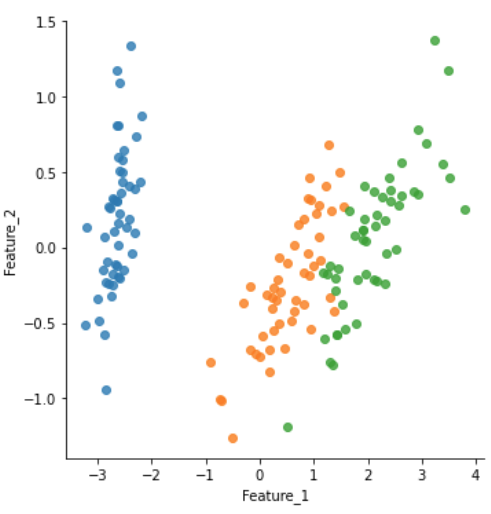
\includegraphics[width=8.0cm]{./pic/Clustering_Beispiel.png}
    \caption{Beispiel für Clustering}
    \label{fig:Clustering_Beispiel}
\end{figure}

Bei der ,,\textit{Dimensionality Reduction}'' versucht der Algorithmus das Datenset in seiner 
Dimensionalität, also in der Anzahl an Feldern, zu reduzieren. Es wird also die Frage gestellt, 
ob sich in einem bestehenden Datenset auch mit weniger Feldern Abhängigkeiten feststellen lassen. Dieser 
Schritt wird vor allem für Modelle benutzt, die sensibel gegenüber hoher Dimensionalitäten sind, 
sodass das Datenset vor dem Training in seiner Dimensionalität heruntergebrochen werden kann.

Im Rahmen des Projektes wurden hauptsächlich Klassifizierungs-Algorithmen genutzt, da ein Großteil der 
Datensets Labels zur Überprüfung hatte.\\
Um einen Vergleich zu ermöglichen, werden später trotzdem noch 
einzelne Ergebnisse von Clustering und Dimensionality Reduction betrachtet. Im Folgenden sollen die genutzten 
Modelle erklärt werden.
\newpage
\subsection{Random Forest Classifier}

\textit{Random Forest Classifier} RFC stellen eine Unterkategorie der ,,\textit{Decision Trees}'' dar. Decision Trees sind einfache
Anordnungen von bestimmten Fragen, die über das Datenset gestellt werden, um eine Klassifikation zu erreichen.

\begin{figure}[h]
    \centering
    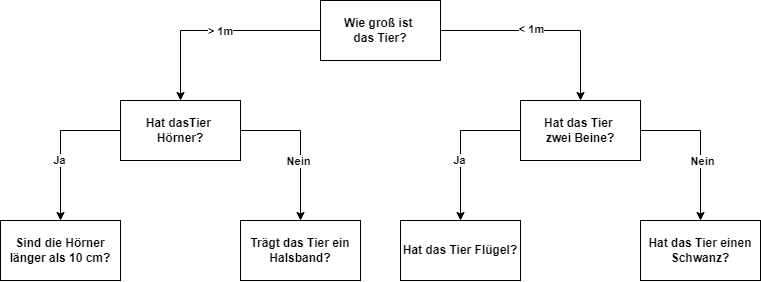
\includegraphics[width=10.0cm]{pic/DecisionTree.png}
    \caption{Beispiel eines Decision Trees}
    \label{fig:DT_Beispiel}
\end{figure}

Erstellt man ein ,,\textit{Ensemble}'' aus Decision Trees, die Erwartungen über einen zufällig gewählten 
Teil des Datensets treffen können, entsteht ein Random Forest.
Der Random Forest Classifier versucht, eine Menge einfacher Schätzfunktionen über einen komplexeren 
Sachverhalt ,,abstimmen'' zu lassen. Während sich in einem einzelnen Entscheidungsbaum Fehleinschätzungen 
entwickeln können, sinkt die Chance auf eine solche Fehleinschätzung, je mehr unabhängige 
Entscheidungsbäume man befragt. 

\subsection{Gradient Boosting Classifier}
Der \textit{Gradient Boosting Classifier} GBC ist eine Abwandlung eines RFC und  versucht, seine Erwartungen
aufgrund von Abweichungen eines Labels vom Durchschnitt dieses Labels zu treffen. \\
Versucht man beispielsweise aus dem Gewicht eines Tieres dessen Alter zu bestimmen, wird 
ein GBC als Ausgangswert den Durchschnitt aller Label-Werte, also dem Gewicht, berechnen. Danach werden die 
Abweichungen aller Label-Werte zu diesem Durchschnitt gebildet. Diese Abweichungen werden nun in Beziehung zu den 
anderen Spalten des Datensets gesetzt. 
\\\\
Beispielsweise könnte man so davon ausgehen, dass ausgewachsene Tiere von einem 
bestimmten Alter über dem Durchschnittsgewicht liegen. Genauso liegen besonders junge Tiere wahrscheinlich immer
einen ähnlichen Wert unter dem Durchschnittsgewicht. So wurde zwischen dem Label \textit{Gewicht} und der Spalte 
\textit{Alter} eine Beziehung hergestellt. In weiteren Iterationen orientiert sich der GBC immer an der Abweichung 
zum Durchschnittswert des vorherigen Baumes. So werden die getroffenen Erwartungen über mehrere Iterationen immer 
präziser.
\newpage
\subsection{Support Vector Classifier}
Der \textit{Support Vector Classifier} SVC versucht in einem Datenset anhand von bestimmten Cut-Off-Values klare Grenzen 
zwischen Werten zu finden, sodass man alle Messwerte ober- und unterhalb der Grenze eindeutig klassifizieren 
kann.

\begin{figure}[h]
    \centering
    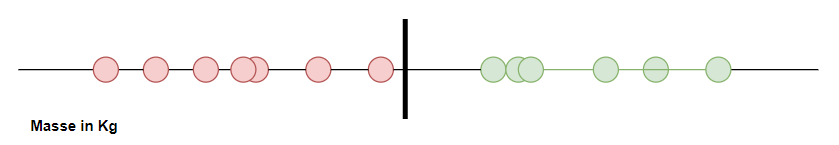
\includegraphics[width=10.0cm]{pic/SVC_1D.png}
    \caption{Beispiel eines Support Vector Classifiers}
    \label{fig:SVC_1D}
\end{figure}

In Abb. \ref{fig:SVC_1D} ist der SVC ein Punkt auf einer eindimensionalen Linie, auf der das Gewicht in kg von z.B. 
Tieren in ,,unter-'' und ,,übergewichtig'' unterteilt wird. Dieser Punkt ist Ergebnis aller Verhältnisse der einzelnen
Datenpunkte zueinander. Durch sog. ,,\textit{Kernel Funktionen}'' versucht der Algorithmus nun Beziehungen 
in höheren Dimensionen zu finden, wie z.B. $Masse^2$, $Masse^3$ usw. . Der SVC stellt dann in diesen Dimensionen 
eine Linie in einem zweidimensionalen oder eine Ebene in einem dreidimensionalen Koordinatensystem dar.\\

\begin{figure}[h]
    \centering
    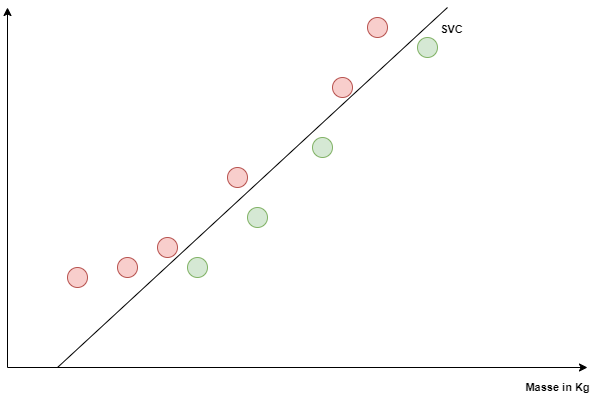
\includegraphics[width=10.0cm]{pic/SVC_2D.png}
    \caption{Beispiel eines Support Vector Classifiers in der zweiten Dimension}
    \label{fig:SVC_2D}
\end{figure}

Da der SVC die Verhältnisse aller Datenpunkte zueinander betrachtet, ist er sehr anfällig für Abweichungen in 
den Daten, was bei der Datenvorbereitung und der Auswertung beachtet werden muss.

\newpage
\subsection{Logistische Regression}

Die \textit{Logistische Regression} LR ordnet Daten anhand einer Wahrscheinlichkeit einem bestimmten Label  zu. Trotz des Teilnamens
,,Regression'' handelt es sich um einen Klassifizierungsalgorithmus. Der Name kommt daher, dass die berechnete Wahrscheinlichkeit
zu einem kontinuierlichen Label zwischen 0 und 1 führt, was durch die Form einer Sigmoid-Funktion ausgedrückt wird.
Der Algorithmus eignet sich wegen dieser Eigenschaft besonders für  das Klassifizierungsproblem der Projektarbeit, 
bei der ein Wahrheitswert, wie ,,Anwesenheit'' oder ,,Abwesenheit'' untersucht werden soll.\\
Nutzt man logistische Regression beispielsweise zur Abbildung einer Beziehung zwischen Gewicht von Tieren in Gramm 
zu einer Wahrscheinlichkeit für Übergewicht, könnte das entstehende Modell wie folgt aussehen.

\begin{figure}[h]
    \centering
    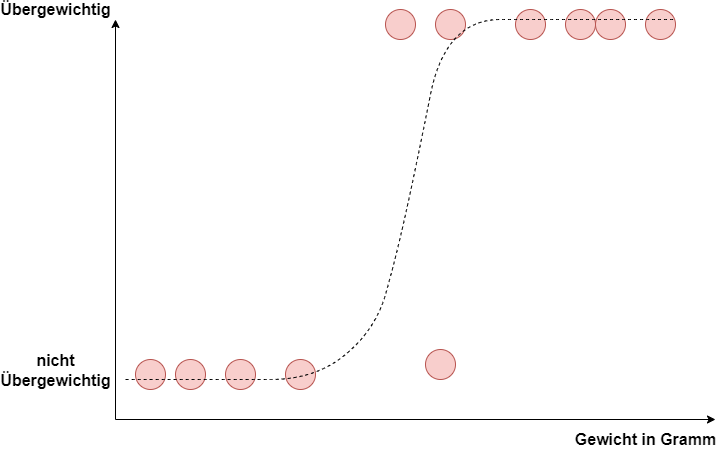
\includegraphics[width=10.0cm]{pic/logistic_regression.png}
    \caption{Beispiel logistischer Regression}
    \label{fig:LR}
\end{figure}

Die Sigmoid-Funktion wird grundsätzlich durch

\begin{align}
    p = \frac{1}{1 + e^{-(x-\mu)/s}}
\end{align}

beschrieben, wobei x der Eingabewert in Gramm darstellt und $\mu$ der Mittelpunkt der Kurve beschreibt, der sich aus dem 
Verhältnis von Eintrittswahrscheinlichkeit $p_1$ und Gegenwahrscheinlichkeit $p_0$ ergibt.

\begin{align}
    p(\mu) = 0.5 = \frac{p_1}{p_0}   
\end{align}

\newpage
Zusätzlich beschreibt s einen Skalierungsparameter, mit dem die Form der Kurve flacher oder steiler werden kann,
was angibt, wie eindeutig die eingegebenen Daten zugeordnet werden können. Wären im o.g. Beispiel also alle roten
Punkte jeweils links und rechts von der Mitte einsortiert, wäre die Sigmoid-Funktion in der Mitte sehr steil, da alle
Daten anhand des Mittelpunktes klar getrennt werden könnten.

\begin{figure}[h]
    \centering
    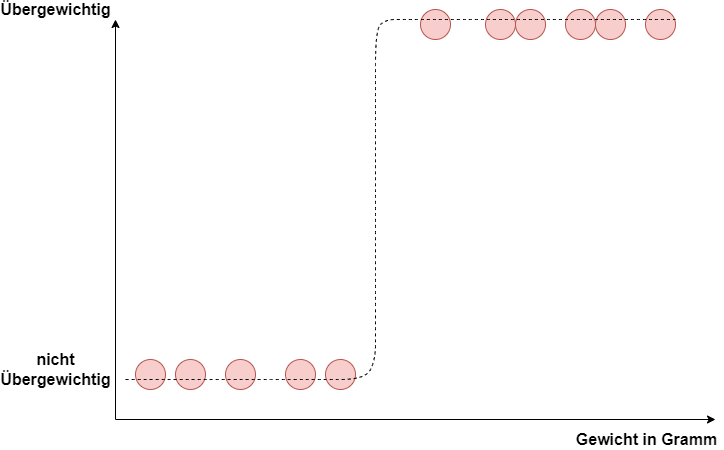
\includegraphics[width=10.0cm]{pic/logistic_regression_high s.png}
    \caption{Logistische Regression mit deutlicher Skalierung}
    \label{fig:LR_scal}
\end{figure}

Anhand der optimierten Sigmoid-Funktion können nun neue Daten klassifiziert werden, wobei die Wahrscheinlichkeit
bei $p < 0.5$ auf 0 und $p >= 0.5$ auf 1 gerundet wird.
\newpage
\subsection{K-Nearest-Neighbours Clustering}
Der \textit{K-Nearest-Neighbours}-Algorithmus KNN betrachtet den Abstand von einem gegebenen Punkt $p$ zu einer 
Menge an Punken in einem Datenset und ordnet ihn gemäß dieser Abstände einer bestimmten Kategorie zu. Die 
Zuordnung geschieht anhand der Kategorie der größten Menge zum nächsten Nachbarn.

\begin{figure}[h]
    \centering
    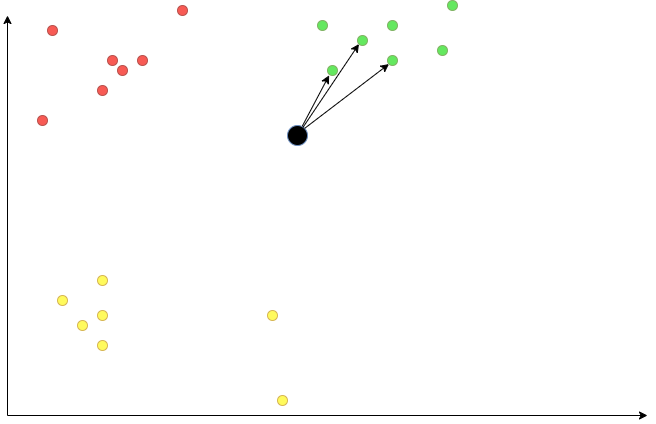
\includegraphics[width=12.0cm]{pic/KNN.png}
    \caption{Beispiel eines KNN}
    \label{fig:KNN}
\end{figure}

Im oben gezeigten Beispiel würde ein Punkt anhand seiner drei nächsten Nachbarn als ,,grün'' kategorisiert.
Die Anzahl der gewünschten Nachbarn, die zu untersuchen sind, ist frei wählbar.
Da die Abstandsberechnung über den \textit{Euklidischen Abstand} berechnet wird, funktioniert dieser 
Algorithmus auch in höheren Dimensionen, denn

\begin{align}
    d = \sqrt{(x2 - x1)^2 + (y2 - y1)^2 + (z2 - z1)^2 + ... + (n2 - n1)^2}
\end{align}

lässt sich für beliebig viele Dimensionen fortsetzen.

\newpage

\subsection{K-Means Clustering}
Der \textit{K-Means} Algorithmus legt eine bestimmte Anzahl von neuen Datenpunkten an eine zufällige Position des
Datensets.  Die herumliegenden Datenpunkte werden nun anhand ihrer Abstände diesen sog. \textit{Clustern} 
zugeordnet (in Abb. \ref{fig:KMeans1} als vertikale Linien dargestellt).\\
Die Abstände werden auch hier durch die Euklidische Abstandsformel berechnet.\\

\begin{figure}[h]
    \centering
    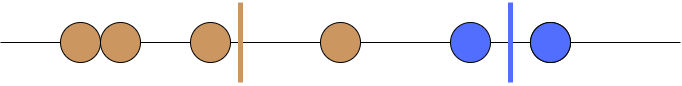
\includegraphics[width=12.0cm]{pic/KMeans_step1.png}
    \caption{Beispiel des K-Means Algorithmus}
    \label{fig:KMeans1}
\end{figure}

Da der Algorithmus die optimale Verteilung von Clustern nicht erkennen kann, wird die Position der Cluster 
gespeichert und neue Cluster an zufällige Positionen gelegt. Sind die durchschnittlichen Abstände der Datenpunkte
zu den neuen Clustern geringer als vorher, werden die gespeicherten Cluster nun in Richtung der neuen Cluster 
verschoben (Abb. \ref{fig:KMeans2}).\\

\begin{figure}[h]
    \centering
    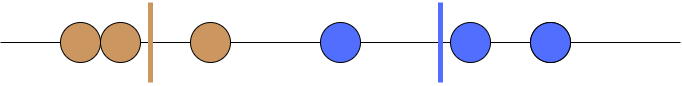
\includegraphics[width=12.0cm]{pic/KMeans_step2.png}
    \caption{Beispiel des K-Means Algorithmus}
    \label{fig:KMeans2}
\end{figure}

Die Anzahl an Schritten die der Algorithmus durchläuft kann vorgegeben werden. Allgemein sollte der Algorithmus
so lange neue Schritte machen, bis der Abstand der gespeicherten und neuen Cluster zueinander einen bestimmten
Minimalwert unterschreitet.

\newpage
\subsection{Neuronale Netzwerke}
Die Funktionsweise eines neuronalen Netzwerks ist direkt angelehnt an die Funktionsweise des menschlichen Gehirns.
Einzelne Knotenpunkte (Neuronen) werden mithilfe von gewichteten Verbindungen verknüpft, sodass das Netzwerk versucht 
Eingabewerte bestimmten Ausgabewerten zuzuordnen. Diese Zuordnung der Ein- und Ausgabewerte im Input- und Output-Layer 
geschieht nicht direkt, sondern durch ein oder mehrere \textit{Hidden Layer}, dessen Neuronenzahl üblicherweise über 
der Anzahl der Neuronen im Input Layer liegt. Die Anzahl der Neuronen im Output-Layer entspricht der Anzahl an Ergebnissen, 
die sich aus dem Input ergeben können. Im Beispiel der Anwesenheitsanalyse entspräche das also zwei Neuronen für 
An- und Abwesenheit.

\begin{figure}[h]
    \centering
    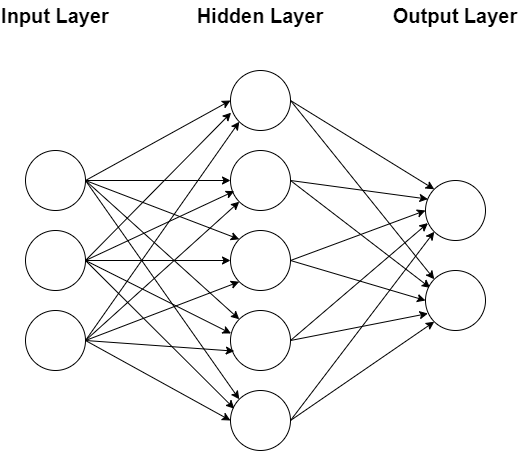
\includegraphics[width=10.0cm]{pic/NN.png}
    \caption{Beispiel eines neuronalen Netzwerks}
    \label{fig:NN}
\end{figure}

Liegt an einem Neuron eine Information an, wird diese als Eingabe einer Aktivierungsfunktion $\varphi$ genutzt, 
die mithilfe eines bestimmten Schwellwertes bestimmt, ob dieses Neuron aufgrund der Eingabe aktiviert wird. Über eine 
bestimmte Anzahl von Iterationen werden die Gewichtungen zwischen den einzelnen Neuronen stärker oder schwächer.


\subsection{Long Short Term Memory}
Das \textit{Long Short Term Memory} LSTM ist eine Abwandlung herkömmlicher neuronaler Netzwerke. Es handelt sich um ein
\textit{rekurrentes} neurales Netzwerk, was bedeutet, dass jedes Neuron seine Ausgabewerte auch wieder als Eingabewerte
nutzt. Der Begriff \textit{Memory} rührt daher, dass durch diese Rückkopplung eine Art Gedächtnis entsteht, durch 
die das Netzwerk bessere Rückschlüsse auf die Einordnung des aktuellen Input-Wertes ziehen kann.\\

\begin{figure}[h]
    \centering
    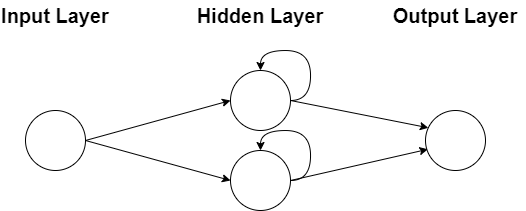
\includegraphics[width=10.0cm]{pic/RecurrentNN.png}
    \caption{Beispiel eines rekurrenten neuronalen Netzwerks}
    \label{fig:RecNN}
\end{figure}
\newpage
Bei einem LSTM verfügt jedes Neuron zusätzlich über einen Zell-Status $C_t$, welcher durch einen Input $x_t$ verändert werden kann.
Auf den Zell-Status nehmen \textit{Input-}, \textit{Forget-} und \textit{Output}-Gates Einfluss. Diese drei Gates
besitzen jeweils ein eigenes neuronales Netzwerk $\sigma$.\\\\
Das Input-Gate bestimmt, ob der Zell-Status anhand des anliegenden Inputs verändert werden darf.
Das Forget-Gate gibt an, ob der Status der Zelle zurückgesetzt und somit das ,,Gedächtnis'' der Zelle gelöscht wird. Es
stellt die zentrale Komponente des LSTMs dar.
Das Output-Gate regelt, ähnlich wie Aktivierungsfunktion normaler NNs, ob der anliegende Input zu einem Output 
der Zelle führt.

\begin{figure}[h]
    \centering
    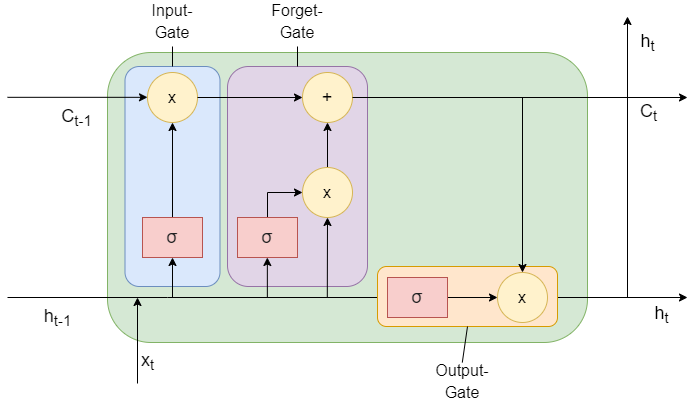
\includegraphics[width=12.0cm]{pic/LSTM-Cell.png}
    \caption{Vereinfachter Aufbau einer LSTM-Zelle}
    \label{fig:LSTM_Cell}
\end{figure}

Ein LSTM kann auf diese Weise eine Vielzahl vorangegangener Zeitschritte einbeziehen. Es verlässt sich so nicht 
direkt auf einen gegebenen Input, sondern auf einen langen Verlauf von bereits verarbeiteten Input-Werten. 
LSTMs sind deshalb besonders interessant für Probleme bei denen Beziehungen zwischen kontinuierlichen 
Datenwerten gebildet werden müssen.

\newpage
Man gehe man von einem LSTM aus, das über eine Liste an Namen verfügt und anhand eines Datensatzes gelernt
hat, zwei Namen mit der Beziehung ,,sah'' zu z.B. ,,Jonas sah Jakob.'' zu verknüpfen.\\
Das LSTM hat nun intern einen Status, der angibt, dass auf einen Namen mit hoher Wahrscheinlichkeit das Wort 
,,sah'' und mit niedriger Wahrscheinlichkeit ein zweiter Name folgt. 
Beginnt man nun einen neuen Satz mit ,,Jakob'', werden als mögliche nächste Worte ,,Jonas'', ,,Jakob'' und ,,sah''
ausgewählt. Bisher ähnelt dieser Verlauf einem normalen neuronalen Netzwerk. Beim LSTM
steht aber nun wegen des vorherigen Durchlaufs der Name ,,Jakob'' im Forget-Gate, sodass ,,Jakob'' aus der verfügbaren
Wortauswahl für das nächste Wort gelöscht wird.\\



\section{CO2 als Anwesenheitsindikator}\label{CO2}

%Der CO2-Gehalt der Raumluft ist als sehr guter Indikator für menschliche Präsenz anzusehen. Anders als andere 
%Umweltindikatoren wie Temperatur oder Luftfeuchtigkeit hat der CO2-Gehalt die Eigenschaft, dass es in 
%geschlossenen Räumen keine äußeren Einflussfaktoren für diesen Messwert gibt. In einem Büroraum kann der 
%Mensch als alleinige Quelle für CO2 angesehen werden.\\
Der Anteil von CO2 in frischer Atemluft beträgt zwischen 350 und 450 ppm. Es gibt in Deutschland und auch Europa 
keine grundsätzlich festgelegten Grenzwerte für akzeptable Raumluft, vielmehr raten Gesundheitsämter 
verschiedener Länder Grenzwerte zwischen 1200 und 1500 ppm einzuhalten. Ab der Obergrenze von 1500 ppm 
zeigen sich beim Menschen erste Müdigkeitserscheinungen, weshalb dieser Wert in der Literatur als maximaler 
Richtwert für Innenräume gilt.\\

\begin{figure}[h]
    \centering
    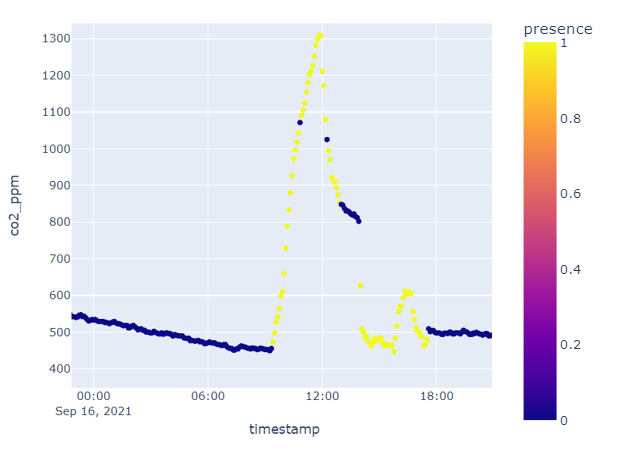
\includegraphics[width=0.7\textwidth]{pic/co2_singleDay.png}
    \caption{CO2-Gehalt der Raumluft über einen Tag}
    \label{fig:CO2_oneDay}
\end{figure}
 
Es ist zu erkennen, dass die CO2-Werte in einem normalen Büroraum innerhalb dieser empfohlenen Grenzen schwanken.
Abgesehen von einigen kleinen Pausen sind fast durchgehend Personen anwesend, die täglich etwa um 12:00 Uhr den 
Raum lüften.
Es ist auch klar zu erkennen, dass sich der CO2-Gehalt während der Abwesenheit von Personen durch die passive
Lüftung des Raumes (Tür-/Fensterspalten) langsam wieder gegen den Grundwert bewegt.

\newpage
\section{Luftfeuchtigkeit und Temperatur}
Auch wenn Luftfeuchtigkeit und Temperatur Indikatoren für menschliche Präsenz in einem Raum sein können, 
unterscheidet sich deren Aussagekraft von der des CO2-Gehaltes der Raumluft in einem wichtigen Faktor.\\ 
Sie werden beide stark von äußeren Umweltfaktoren wie dem aktuellen Wetter oder der Jahreszeit beeinflusst.
Beide Werte wurden zunächst in das Training aller Modelle miteinbezogen; es wird allerdings im folgenden 
Kapitel gezeigt, dass diese beiden Werte zusammen mit dem CO2-Wert wenig aussagefähig sind und 
deshalb später nicht weiter genutzt werden.  

\section{Sensordaten}
Wie bereits beschrieben, wurden die Sensordaten in mehreren Räumen der FH Aachen kontinuierlich 
gesammelt. Durch das Filtern nach den einzelnen Räumen kann für jeden Raum ein Datenset nach folgender Struktur
erzeugt werden:\\

\begin{table}[ht]
    \caption{Sensordaten}
    \centering
    \begin{tabular}{|p{4.5cm}||p{3cm}|p{5.5cm}|}
        \hline
        \multicolumn{3}{|c|}{Sensordaten} \\
        \hline
        Name&Format &Beschreibung\\
        \hline
        timestamp&timestamp&Zeitpunkt der Messung\\
        co2\_ppm&integer&CO2-Wert\\
        temperature\_celsius&float&Temperatur in Grad Celsius\\
        relative\_humidity\_percent&float&Luftfeuchtigkeit\\
        presence&boolean&Aktivität Bewegungssensor\\
        \hline
    \end{tabular}             
\end{table}

\newpage
\chapter{Technische Umsetzung}

\section{Datenbeschaffung und -Vorbereitung}
Die Daten wurden lokal auf einem der FH-Server in Form eines \textit{Hadoop Distributed File System} (HDFS) 
gespeichert. Mithilfe von Apache Drill waren die Daten jederzeit durch einfache SQL-Abfragen abrufbar. 
Die Daten wurden so während der gesamten Dauer des Projektes immer aktuell gehalten, damit alle Erkenntnisse 
jeweils auf der aktuellsten Datenlage basieren.
\\\\
Die Datenvorbereitung (Pre-Processing) ist einer der wichtigsten Schritte bei der Anwendung von Machine 
Learning. Dadurch besteht die Möglichkeit, beim Training des Modells durch Bearbeitung bestehender Spalten
oder Hinzufügen zusätzlicher Spalten im Datenset Schwerpunkte zu setzen, die es den Algorithmen beim Training
zum einen erleichtern, ihre Erwartungen zu präzisieren, zum anderen aber auch deren Leistung bei der Verarbeitung
bestimmter Spalten zu steigern.
\subsection{Gruppierung}
Die Sensordaten wurden alle sechs Sekunden erfasst. Da sich weder CO2-Gehalt noch Feuchtigkeits- oder 
Temperaturwerte der Raumluft so schnell nicht verändern, wurden die Daten direkt beim Drill per SQL zu 
zwei-Minuten-Intervallen zusammengefasst. Dabei werden über alle Spalten hinweg Durchschnittswerte gebildet, 
die dann zu einem Datensatz zusammengefasst werden. 
Dies steigert die Leistung aller Algorithmen erheblich, weil sich dadurch die Zahl der 
Datensätze stark verringert. Da sich, wie oben erwähnt, der CO2-Gehalt der Raumluft in einem 
Intervall von zwei Minuten kaum merklich verändert, verringert sich die Genauigkeit des gesamten Datensets
dadurch nicht maßgeblich.
\subsection{Zyklische Codierung}
Zyklische Codierung wird immer dort verwendet, wo Daten sich in wiederholenden Schemata bewegen. Diese 
Schemata, wie z.B. die Zahlenumbrüche bei einer Uhrzeit, sind für Algorithmen nicht direkt ersichtlich und 
sind zudem für Computer nicht leicht zu verarbeiten. Durch eine Encodierung in 
Sinus- und Cosinus-Werte können diese Zusammenhänge vereinfacht werden.\\
Hierzu wurde der Timestamp zuerst in Sekunden übersetzt, sodass sich ein bestimmter Zeitpunkt eines Tages 
immer zwischen 0 und 86399 Sekunden bewegt.
Aus diesem Wert wurden dann zwei neue Datenspalten ,,\textit{hour\_sin}'' und ,,\textit{hour\_cos}'' 
in das Datenset eingefügt, welche sich aus 

\begin{align}
    hour\_sin = sin(2 * \pi * x / x_{max}) \\ 
    hour\_cos = cos(2 * \pi * x / x_{max})
\end{align} 

ergeben. So kann jede Tageszeit einer eindeutigen Kombination aus Sinus- und Cosinus-Werten zwischen 
$0$ und $1$ zugeordnet werden.

\subsection{Deltas und Shift-Werte}
Desweiteren wurden von den Spalten ,,\textit{co2\_ppm}'', ,,\textit{temperature\_celsius}'' und \break 
,,\textit{relative\_humidity\_percent}'', die tatsächlich Rückschlüsse auf die Präsenz zulassen, \break 
zusätzliche Delta- und Shift-Spalten angelegt.\\\\
Ein Shift-Wert bedeutet lediglich, dass  in einer Zeile $x_n$ des Datensets 
zusätzlich, neben den aktuellen Werten, auch Werte von $k$ Zeilen zuvor, also $x_{n-k}$ stehen. So haben 
alle Algorithmen direkten Zugriff auf Vergangenheitswerte der ausgewählten Spalten.\\\\
Delta-Spalten stellen, dem Namen nach, Deltas zu vorherigen Werten dar:

\begin{align}
    \Delta x_k = x_n - x_{n-k}    
\end{align}

Die Erwartung ist hier, dass die Änderung der CO2-, Temperatur- und 
Luftfeuchtigkeitswerte ein wichtigerer Indikator sein könnte, als die tatsächlichen Werte. In einem schlecht 
klimatisierten Raum könnten Grundwerte von z.B. CO2 höher sein, als in Räumen, in denen regelmäßig gelüftet wird.
Unabhängig dieser Grundwerte könnte man bei einem starken Anstieg wesentlich einfacher menschliche Präsenz erkennen, 
ohne dass zunächst die vorangegangenen Werte überprüft werden müssen.
Durch die hinzufügten 
Deltas werden diese Grundwerte ignoriert und Rückschlüsse auf die aktuelle Präsenz sind besser möglich.\\
Im Zuge der Projektarbeit wurden verschiedene Kombinationsmöglichkeiten von Delta- und Shiftwerten mit 
Zeitschritten zwischen zwei Minuten und einer Stunde mit Hinblick auf Verbesserungen der Modell-Genauigkeiten 
getestet.

\subsection{Outlier Detection}
Wie bereits erwähnt, spielen Datenausreißer für die Ergebnisse mancher Algorithmen eine große Rolle. Überall 
wo z.B. aus einer Reihe von Datenwerten Durchschnittswerte berechnet werden, würden Ausreißer in den Daten das 
Ergebnis verfälschen und die Aussagekraft des Algorithmus deutlich senken.
Um diese Ausreißer vor dem Training der Modelle zu beseitigen, wurde das Verfahren des 
\textit{Interquartilabstands} (IQR nach der englischen Bezeichnung \textit{Interquartile Range}) gewählt.\\
Der IQR gibt die Intervallgröße an, die ein Wert vom Median einer Datenreihe abweichen darf. Bei einer 
der Größe nach sortierten Datenreihe $x = (x_0,x_1,...,x_n)$ bestimmt man die Mediane der unteren und oberen 
Hälfe des Datensets $Q_1$ und $Q_2$. Der IQR ergibt sich nun aus 
\begin{align}
    IQR = Q_2 - Q_1
\end{align}
Mit diesm Wert können jetzt die erlaubten Ober- und Untergrenzen 
des Datensets mit 
\begin{align}
    Limit_{upper} = Q_2 + 1.5 * IQR \\
    Limit_{lower} = Q_1 - 1.5 * IQR
\end{align} 
bestimmt werden. Alle Werte die außerhalb dieser Grenzen liegen, können als Ausreißer betrachtet werden.\\
Ausreißer zu entfernen, ist hier wichtig, da die Sensoren Messfehler erzeugen können und einige Modelle dadurch,
wie bereits beschrieben, stark beeinflusst werden können.

\section{Validierung}
\sloppy
Über das Projekt hinweg wurden verschiedene Validierungsmethoden verwendet. Grundsätzlich unterteilt man das 
Datenset in ein Trainings- und Testset mit einem Verhältnis von etwa 80-20. Das bedeutet, dass das Modell mit
80 Prozent der Daten trainiert wird, wobei die anderen 20 Prozent zurückgehalten werden, um daraufhin das 
fertig trainierte Modell daran zu testen. Aus dem Ergebnis dieses Tests ergeben sich verschiedene Werte, die  
die allgemeine Genauigkeit des Modells repräsentieren, d.h. wie verlässlich das Modell die An- und Abwesenheit 
des Testsets selbst berechnen kann, wenn man ihm den tatsächlichen Wert vorenthält.\\
Allgemeine Basis für die errechneten Genauigkeiten bildet die sog. \textit{Confusion Matrix}.

\begin{figure}[h]
    \centering
    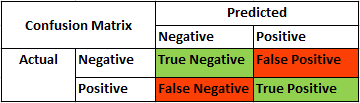
\includegraphics[width=0.6\textwidth]{pic/confusion_matrix_ex.png}
    \caption{Beispiel einer Confusion Matrix}
    \label{fig:CV}
\end{figure}

Diese zeigt, inwiefern die Genauigkeit des Modells neben tatsächlich richtig erkannten Werten zusätzlich
von false negatives und false positives beeinflusst wird.\\
\newpage
Die \textit{Accuracy Score} ist eine einfache Methode zur Bestimmung der Modellqualität und berechnet sich 
aus der Summe der richtigen Ergebnisse geteilt durch die Summe aller Ergebnisse.

\begin{center}
    $AccuracyScore = \dfrac{TP + TN}{TP + TN + FP + FN}$    
\end{center}
Die \textit{Recall Score} beschreibt die Genauigkeit bezogen auf alle erkannten positiven Ergebniswerte. 
%Dabei ist wichtig, dass wenn ein Algorithmus beispielsweise Anwesenheit zu erkennen versucht auch ein
%false negative als Treffer gewertet wird.
\begin{center}
    $RecallScore = \dfrac{TP}{TP + FN}$    
\end{center}

Die \textit{Precision Score} gibt die allgemeine Menge an positiven Werten an, die hätten erkannt werden müssen.
\begin{center}
    $PrecisionScore = \dfrac{TP}{TP + FP}$    
\end{center}

Die \textit{F1-Score} ist der Durchschnittswert aus Recall- und Precision-Score und liefert im Allgemeinen eine 
gute Auskunft über die Qualität eines Modells.\\

\begin{center}
    $F1\_Score = \dfrac{2}{\dfrac{1}{PrecisionScore} + \dfrac{1}{RecallScore}} = \dfrac{2 \cdot (PrecisionScore \cdot RecallScore)}{PrecisionScore + RecallScore}$    
\end{center}

\vspace{0.75cm}
In diesem Anwendungsfall ist es durchaus wichtig, Werte zur Anwesenheit von Personen genauer zu betrachten als 
Werte zur Abwesenheit, da die tägliche Arbeitszeit nur etwa ein Drittel eines ganzen Tages ausmacht. 
Da von 24 Stunden ca. 16 Stunden Werte zur Abwesenheit und nur etwa 8 Stunden Werte zur Anwesenheit enthalten, 
ist das Datenset also mit einem Verhältnis von etwa 1/3 in Richtung der Abwesenheit unausgeglichen. 
Dies lässt die Erwartung zu, dass das trainierte Modell wesentlich besser darin sein wird, Abwesenheit von Personen
zu erkennen, als Anwesenheit.\\
Hierzu wurde bei der Auswertung der Ergebnisse immer auch der \textit{Classification Report} hinzugezogen,
aus dem ersichtlich ist, wie genau das Modell beide möglichen Labelwerte berrechnen konnte.
\newpage
Desweiteren war es entscheidend zu erkennen, dass das Datenset über mehrere Monate hinweg nicht perfekt uniform 
ist, da in bestimmten Monaten verhältnismäßig viele Urlaubstage (z.B. Weihnachten/Silvester) vorkommen und es damit 
zu einer Häufung an Abwesenheitswerten kommt.
Wenn die Daten nun im o.g. Verhältnis aufgeteilt werden und dann viele Daten des Testsets in solchen Monaten 
liegen, könnte es beim Ergebnis zu Verzerrungen kommen.\\
Hierfür wurde eine \textit{Kreuzvalidierung} (engl. Cross Validation CV) implementiert. Bei einer CV wird das 
Datenset immer noch im gleichen Verhältnis aufgeteilt, allerdings mehrmals, sodass die Trainings- und Testsets 
jedes Mal aus jeweils anderen Daten bestehen.

\begin{figure}[h]
    \centering
    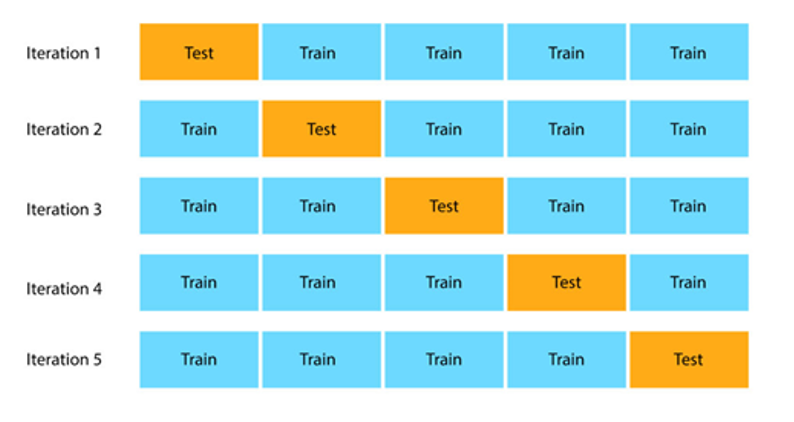
\includegraphics[width=0.7\textwidth]{pic/CV.png}
    \caption{Beispiel einer Kreuzvalidierung}
    \label{fig:CV}
\end{figure}

Errechnet man nun die Durchschnittsgenauigkeit aller Iterationen der CV, ergibt sich eine Gesamtgenauigkeit, 
die das Model besser repräsentiert, weil es mit einer größeren Anzahl von verschiedenen Daten trainiert und 
getestet wurde.
\\\\
Da es für manche Räume keine Datensätze mit Labelwerten gab, musste die Validierung dieser Datensätze 
augenscheinlich erfolgen. Hierfür wurde in ein Datenset eine Labelspalte eingefügt, die dann vom trainierten
Modell selbst gefüllt werden sollte. Das Ergebnis musste schließlich als Graph gezeichnet und per Hand validiert 
werden. Da sich das Ergebnis der Berechnung in diesem Anwendungsfall, wie oben gezeigt, sehr übersichtlich als 
Graph darstellen lässt, war diese Methode der Validierung zwar nicht perfekt, lieferte aber trotzdem einen 
ausreichenden Eindruck über die Qualität des trainierten Modells.


\subsection{Over- und Underfitting}
Over- und Underfitting sind Probleme, die bei allen Machine Learning Algorithmen auftreten können und bezeichnen 
im Allgemeinen einen falschen Umgang mit dem Datenset.
\textit{Overfitting} bedeutet, dass das Modell mit zu vielen, sich zu stark ähnelnden, Daten trainiert wurde, 
wodurch es in der Lage ist, nur neue Daten richtig zu kategorisieren, die dem Trainingsset besonders ähnlich sind.
Overfitting kann während einer Kreuzvalidierung oder der Validierung anhand eines anderen Datensets als dem 
Trainingsset erkannt werden.\\
Um Overfitting zu verhindern, kann das Datenset vereinfacht werden, um so die Beziehungen zwischen den
für die Erwartungsberechnung relevanten Spalten zu stärken.\\\\
\textit{Underfitting} bedeutet dagegen, dass es das Modell nicht geschafft hat, zwischen den gegebenen Daten
Beziehungen herzustellen, sodass das Modell unbekannte Daten richtig kategorisieren kann. Hier reicht es 
normalerweise aus, dem Modell mehr Daten zur Verfügung zu stellen und in der Datenvorbereitung Felder 
einzufügen, die dem Modell bestimmte Beziehungen zwischen Datenfeldern hervorheben sollen. 

\subsection{Parameter Tuning}
\textit{Parameter Tuning} beschreibt einen Schritt der Modell-Optimierung, der normalerweise stattfindet, 
nachdem ein funktionierendes Modell erstellt wurde, das mit bereits verarbeiteten Daten gute Ergebnisse liefert.
Jedes Modell besitzt Parameter, die bei der Erstellung festgesetzt werden. Diese Parameter haben 
großen Einfluss auf den Trainingsprozess, weshalb es sich anbietet, die Genauigkeiten mehrerer Modelle 
mit verschiedenen Parameter-Kombinationen zu testen.\\
Das im Scikit-Learn enthaltene \textit{GridSearchCV}-Modul
bietet die Möglichkeit, einem Modell eine Vielzahl von verschiedenen Parameter-Optionen zu übergeben. Mit diesen 
werden dann automatisch Modelle trainiert und per Kreuzvalidierung verglichen. Am Ende liefert das Modul 
die Parameter-Kombination, mit der das beste Ergebnis erzielt wurde.\\

\begin{figure}[h]
    \centering
    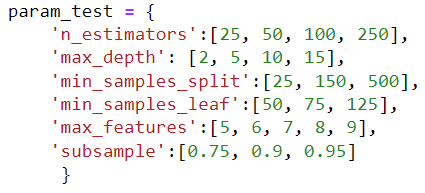
\includegraphics[width=0.6\textwidth]{pic/param_test.png}
    \caption{Beispiel einer Sammlung von Parameter-Optionen}
    \label{fig:Param_Test}
\end{figure}

Im obenstehenden Beispiel kann man erkennen, dass für bestimmte Parameter (rot) eine Sammlung an erlaubten 
Werten (grün) übergeben wird. Alle Kombinationen aus diesen Parameter-Optionen werden dann vom 
GridSearchCV-Modul ausgewertet.\\
Die Verbesserungen gegenüber Standard-Parametern bewegen sich normalerweise im niedrigen einstelligen 
Prozent-Bereich.
%% Zwei Abbildungen, die zusammen gehören

%\begin{figure}
%        \centering
%        \begin{minipage}[c]{0.45\textwidth}
%                \includegraphics[height=6.5cm]{pic/dateiname1.png}
%        \end{minipage}
%        \begin{minipage}[c]{0.45\textwidth}
%                \includegraphics[height=6.5cm]{pic/dateiname2.png}
%        \end{minipage}
%        \caption{Zwei Abbildungen}\label{fig:zwei_abb}
%\end{figure}
